%%%%%%%%%%%%%%%%%%%%%%%%%%%%%%%%%%%%%%%%%
% Beamer Presentation
% LaTeX Template
% Version 1.0 (10/11/12)
%
% This template has been downloaded from:
% http://www.LaTeXTemplates.com
%
% License:
% CC BY-NC-SA 3.0 (http://creativecommons.org/licenses/by-nc-sa/3.0/)
%
%%%%%%%%%%%%%%%%%%%%%%%%%%%%%%%%%%%%%%%%%

%----------------------------------------------------------------------------------------
%	PACKAGES AND THEMES
%----------------------------------------------------------------------------------------

\documentclass{beamer}

\mode<presentation> {

% The Beamer class comes with a number of default slide themes
% which change the colors and layouts of slides. Below this is a list
% of all the themes, uncomment each in turn to see what they look like.

%\usetheme{default}
%\usetheme{AnnArbor}
%\usetheme{Antibes}
%\usetheme{Bergen}
%\usetheme{Berkeley}
%\usetheme{Berlin}
%\usetheme{Boadilla} %like
%\usetheme{CambridgeUS}
%\usetheme{Copenhagen}
%\usetheme{Darmstadt}
%\usetheme{Dresden}
%\usetheme{Frankfurt}
%\usetheme{Goettingen} %like
\usetheme{Hannover} %like
%\usetheme{Ilmenau}
%\usetheme{JuanLesPins}
%\usetheme{Luebeck}
%\usetheme{Madrid}
%\usetheme{Malmoe}
%\usetheme{Marburg}
%\usetheme{Montpellier}
%\usetheme{PaloAlto}
%\usetheme{Pittsburgh}
%\usetheme{Rochester}
%\usetheme{Singapore}
%\usetheme{Szeged}
%\usetheme{Warsaw}

% As well as themes, the Beamer class has a number of color themes
% for any slide theme. Uncomment each of these in turn to see how it
% changes the colors of your current slide theme.

%\usecolortheme{albatross}
%\usecolortheme{beaver}
%\usecolortheme{beetle}
%\usecolortheme{crane}
%\usecolortheme{dolphin}
%\usecolortheme{dove}
%\usecolortheme{fly}
%\usecolortheme{lily}
%\usecolortheme{orchid}
%\usecolortheme{rose}
%\usecolortheme{seagull}
%\usecolortheme{seahorse}
%\usecolortheme{whale}
%\usecolortheme{wolverine}

%\setbeamertemplate{footline} % To remove the footer line in all slides uncomment this line
%\setbeamertemplate{footline}[page number] % To replace the footer line in all slides with a simple slide count uncomment this line

%\setbeamertemplate{navigation symbols}{} % To remove the navigation symbols from the bottom of all slides uncomment this line
}

\usepackage{graphicx} % Allows including images
\usepackage{booktabs} % Allows the use of \toprule, \midrule and \bottomrule in tables
\usepackage{pgfpages}
\usepackage{amsmath}
\usepackage{pgfplots}
\usepackage{tikz}

%----------------------------------------------------------------------------------------
%	TITLE PAGE
%----------------------------------------------------------------------------------------

\title[Computation \& optimization]{Computation \& optimization for Lasso - part 2} % The short title appears at the bottom of every slide, the full title is only on the title page

\author{Luyang Han \& Janosch Ott} % Your name
\institute[] % Your institution as it will appear on the bottom of every slide, may be shorthand to save space
{
ETH Zürich \\ % Your institution for the title page
%\medskip
%\textit{john@smith.com} % Your email address
}
\date{22 October 2018} % Date, can be changed to a custom date

\setbeamercovered{transparent} % else hidden elements are gray, this way they are invisible
\setbeamertemplate{navigation symbols}{} %comment to have a lot of navigating symbols
\setbeamertemplate{section in toc}[sections numbered] % removes the ugly balls
%\setbeameroption{show notes}
\setbeameroption{show notes on second screen=right}
\setbeamertemplate{enumerate items}[default] % to get rid of some more ugly balls


%%%%%%%% ------------%%%%%%%%%%-----------%%%%%%%%%%%------------%%%%%%%%%%-----------
\newcommand{\R}{\mathbb{R}}
\newcommand{\Norm}[1]{\left\lVert#1\right\rVert}
\newcommand{\norm}[1]{\left\lvert#1\right\rvert}
\DeclareMathOperator*{\argmin}{arg\,min}
\DeclareMathOperator*{\argmax}{arg\,max}



%%%%%%%%%%% ----------%%%%%%%%%%-----------%%%%%%%%%%------------%%%%%%%%%--------------


\usepackage{hyperref}



\begin{document}

\begin{frame}
\titlepage % Print the title page as the first slide
\end{frame}

\begin{frame}
\frametitle{Overview} % Table of contents slide, comment this block out to remove it
\tableofcontents % Throughout your presentation, if you choose to use \section{} and \subsection{} commands, these will automatically be printed on this slide as an overview of your presentation
\end{frame}

%----------------------------------------------------------------------------------------
%	PRESENTATION SLIDES
%----------------------------------------------------------------------------------------

%------------------------------------------------
\section{Coordinate Descent}
%------------------------------------------------



%------------------------------------------------
\section{A Simulation Study}
%------------------------------------------------



%------------------------------------------------
\section{Least Angle Regression}
%------------------------------------------------




%------------------------------------------------
\section{Digression: Duality}
%------------------------------------------------

\begin{frame}
\frametitle{Digression: Duality in optimization}

%\begin{tabular}{lcc}
%\toprule
%&Primal&Dual\\\midrule
%Optimize&$\min f(x)$&$\max q(\lambda,\mu)$\\\midrule
%Constraints&$g_i(x)\le0, h_j(x)=0, x\in X$&$\lambda\ge0$\\\midrule
%Function&$L(x,\lambda,\mu):=f(x)+\sum_i\lambda_i g_i(x)+\sum_j\mu_j h_j(x)$&$q(\lambda,\mu)=\inf\limits_{x\in X} L(x,\lambda,\mu)$\\
%&$L(x,\lambda,\mu):=f(x)+\lambda^Tg(x)+\mu^T h(x)$&\\\midrule
%\end{tabular}



%\vspace{15pt}
%Why though? - \textbf{Dual problem is always convex!}

\end{frame}
\note{In various section, I came across terms like "dual" and "dual problem"}

\begin{frame}
\begin{tabular}{ll}
\toprule[1.5pt]
\multicolumn{2}{c}{Primal}\\\midrule
Optimize&$\min f(x)$\\\midrule
Constraints&$g_i(x)\le0, h_j(x)=0, x\in X$\\\midrule
Function&$L(x,\lambda,\mu):=f(x)+\sum_i\lambda_i g_i(x)+\sum_j\mu_j h_j(x)$\\\midrule
%&$L(x,\lambda,\mu):=f(x)+\lambda^Tg(x)+\mu^T h(x)$\\\midrule
\multicolumn{2}{c}{Dual}\\\midrule
Function&$q(\lambda,\mu)=\inf\limits_{x\in X} L(x,\lambda,\mu)$\\\midrule
Constraints&$\lambda\ge0$\\\midrule
Optimize&$\max q(\lambda,\mu)$\\\midrule
\end{tabular}
\vspace{15pt}

Why though? - \textbf{Dual problem is always convex!}

\end{frame}

\note{
$x\in X$ for e.g. solutions in a cone or integer solutions

%$g$ and $h$ are now in vector notation

Terms: Primal problem, Lagrange function with dual variables/Lagrange-multipliers, dual function, dual problem


Dual problem is always convex! - I don't know much about optimization yet, but
they really like convexity.

The second advantage is that all local optima are global optima. That allows local search algorithms to guarantee optimal solutions. And local search is often faster.

(Convexity confers two advantages. The first is that, in a constrained problem, a convex feasible region makes it easier to ensure that you do not generate infeasible solutions while searching for an optimum.)

}



%------------------------------------------------
\section{ADMM}
%------------------------------------------------

\begin{frame}
\frametitle{Alternating Direction Method of Multipliers (ADMM)}
Problem 
\[\underset{\beta\in\R^m, \theta\in\R^n}{\text{minimize}}f(\beta)+g(\theta)\quad\text{subject to}\ \mathbf{A}\beta+\mathbf{B}\theta=c\]
Lagrangian 
\[f(\beta)+g(\theta)+\rho||\mathbf{A}\beta+\mathbf{B}\theta-c||_2^2\]
Augmented Lagrangian
\[L_{\rho}(\beta,\theta,\mu):=f(\beta)+g(\theta)+\left\langle\mu,\mathbf{A}\beta+\mathbf{B}\theta-c\right\rangle+\frac{\rho}{2}||\mathbf{A}\beta+\mathbf{B}\theta-c||_2^2\]
\end{frame}

\note{
Method of Multipliers b/c $\rho$ und $\mu$

Augmented: scalar product with $\mu$ gets added


}

\begin{frame}
\frametitle{Dual Ascent Step}
\framesubtitle{Alternating Direction Method of Multipliers}
\begin{align*}
\beta^{t+1}&=\argmin_{\beta\in\R^m}L_{\rho}(\beta,\theta^t,\mu^t)\\
\theta^{t+1}&=\argmin_{\theta\in\R^m}L_{\rho}(\beta^{t+1},\theta,\mu^t)\\
\mu^{t+1}&=\mu^t+\rho(\mathbf{A}\beta^{t+1}+\mathbf{B}\theta^{t+1}-c)
\end{align*}

\begin{figure}
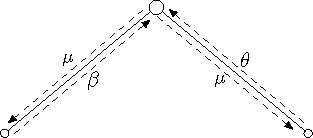
\includegraphics{img/dualascentstep.pdf}
\caption{My own illustration of the dual ascent step in the ADMM algorithm utilising dual decomposition according to \cite{GT12}.}
\end{figure}

\end{frame}

\note{
first two steps is why it is called alternating direction ... cause once we do it in the $\beta$ and once we do it in the $\theta$ direction

last step is called a dual variable update, this dual has nothing to do with two, but is connected to what is called a dual problem

dual ascent step, we are working in the dual problem as "min L", thus convex problem, thus "dual decomposition" into subproblems which is possible by "18-dual-uses.pdf",p. 22, 

think of it as only the last line, sending $\mu$ to the updaters for $\beta$ and $\theta$
}

\begin{frame}
\frametitle{ADMM - Why?}
\begin{itemize}
\item[-] convex problems with nondifferentiable constraints
\item[-] blockwise computation
	\begin{itemize}
	\item[-] sample blocks
	\item[-] feature blocks
	\end{itemize}
\end{itemize}
\end{frame}

\note{
Detailsfor blockwise computation in Exercise 5.12.
}

\begin{frame}
\frametitle{ADMM for the Lasso}
Problem in Lagrangian form
\[\underset{\beta\in\R^p,\theta\in\R^p}{\text{minimize}}\left\{\frac{1}{2}\Norm{\mathbf{y}-\mathbf{X}\beta}_2^2+\lambda\Norm{\theta}_1\right\}\quad \text{such that}\ \beta-\theta=0 \]
Update
\begin{align*}
\beta^{t+1}&=(\mathbf{X}^T\mathbf{X}+\rho\mathbf{I})^{-1}(\mathbf{X}^T\mathbf{y}+\rho\theta^t-\mu^t)\\
\theta^{t+1}&=\mathcal{S}_{\lambda/\rho}(\beta^{t+1}+\mu^t/\rho)\\
\mu^{t+1}&=\mu^t+\rho(\beta^{t+1}-\theta^{t+1})
\end{align*}
where $\mathcal{S}_{\lambda/\rho}(z)=\text{sign}(z)(\norm{z}-\frac{\lambda}{\rho})_+$.
% soft-thresholding parameter
\end{frame}

\note{
Computational cost: Initially $\mathcal{O}(p^3)$, which is a lot, for the SVD(singular value decomposition of $\mathbf{X}$), after that comparable to coordinate descent or composite gradient from earlier
}

%------------------------------------------------
\section{Minor-Max Algorithms}
%------------------------------------------------

\begin{frame}
\frametitle{Minorization-Maximization Algorithms (MMA)}
\begin{itemize}
\item[-] Problem: minimize $f(\beta)$ over $\beta\in\R^p$\\ for $f$ possibly non-convex
\item[-] Introduce additional variable $\theta$
\item[-] Use $\theta$ to majorize (bound from above) the objective function to be minimized
\end{itemize}






{\small Majorization-Minimization Algorithms work analoguosly.}
\end{frame}

\begin{frame}
\frametitle{MMA visually}
\begin{figure}
%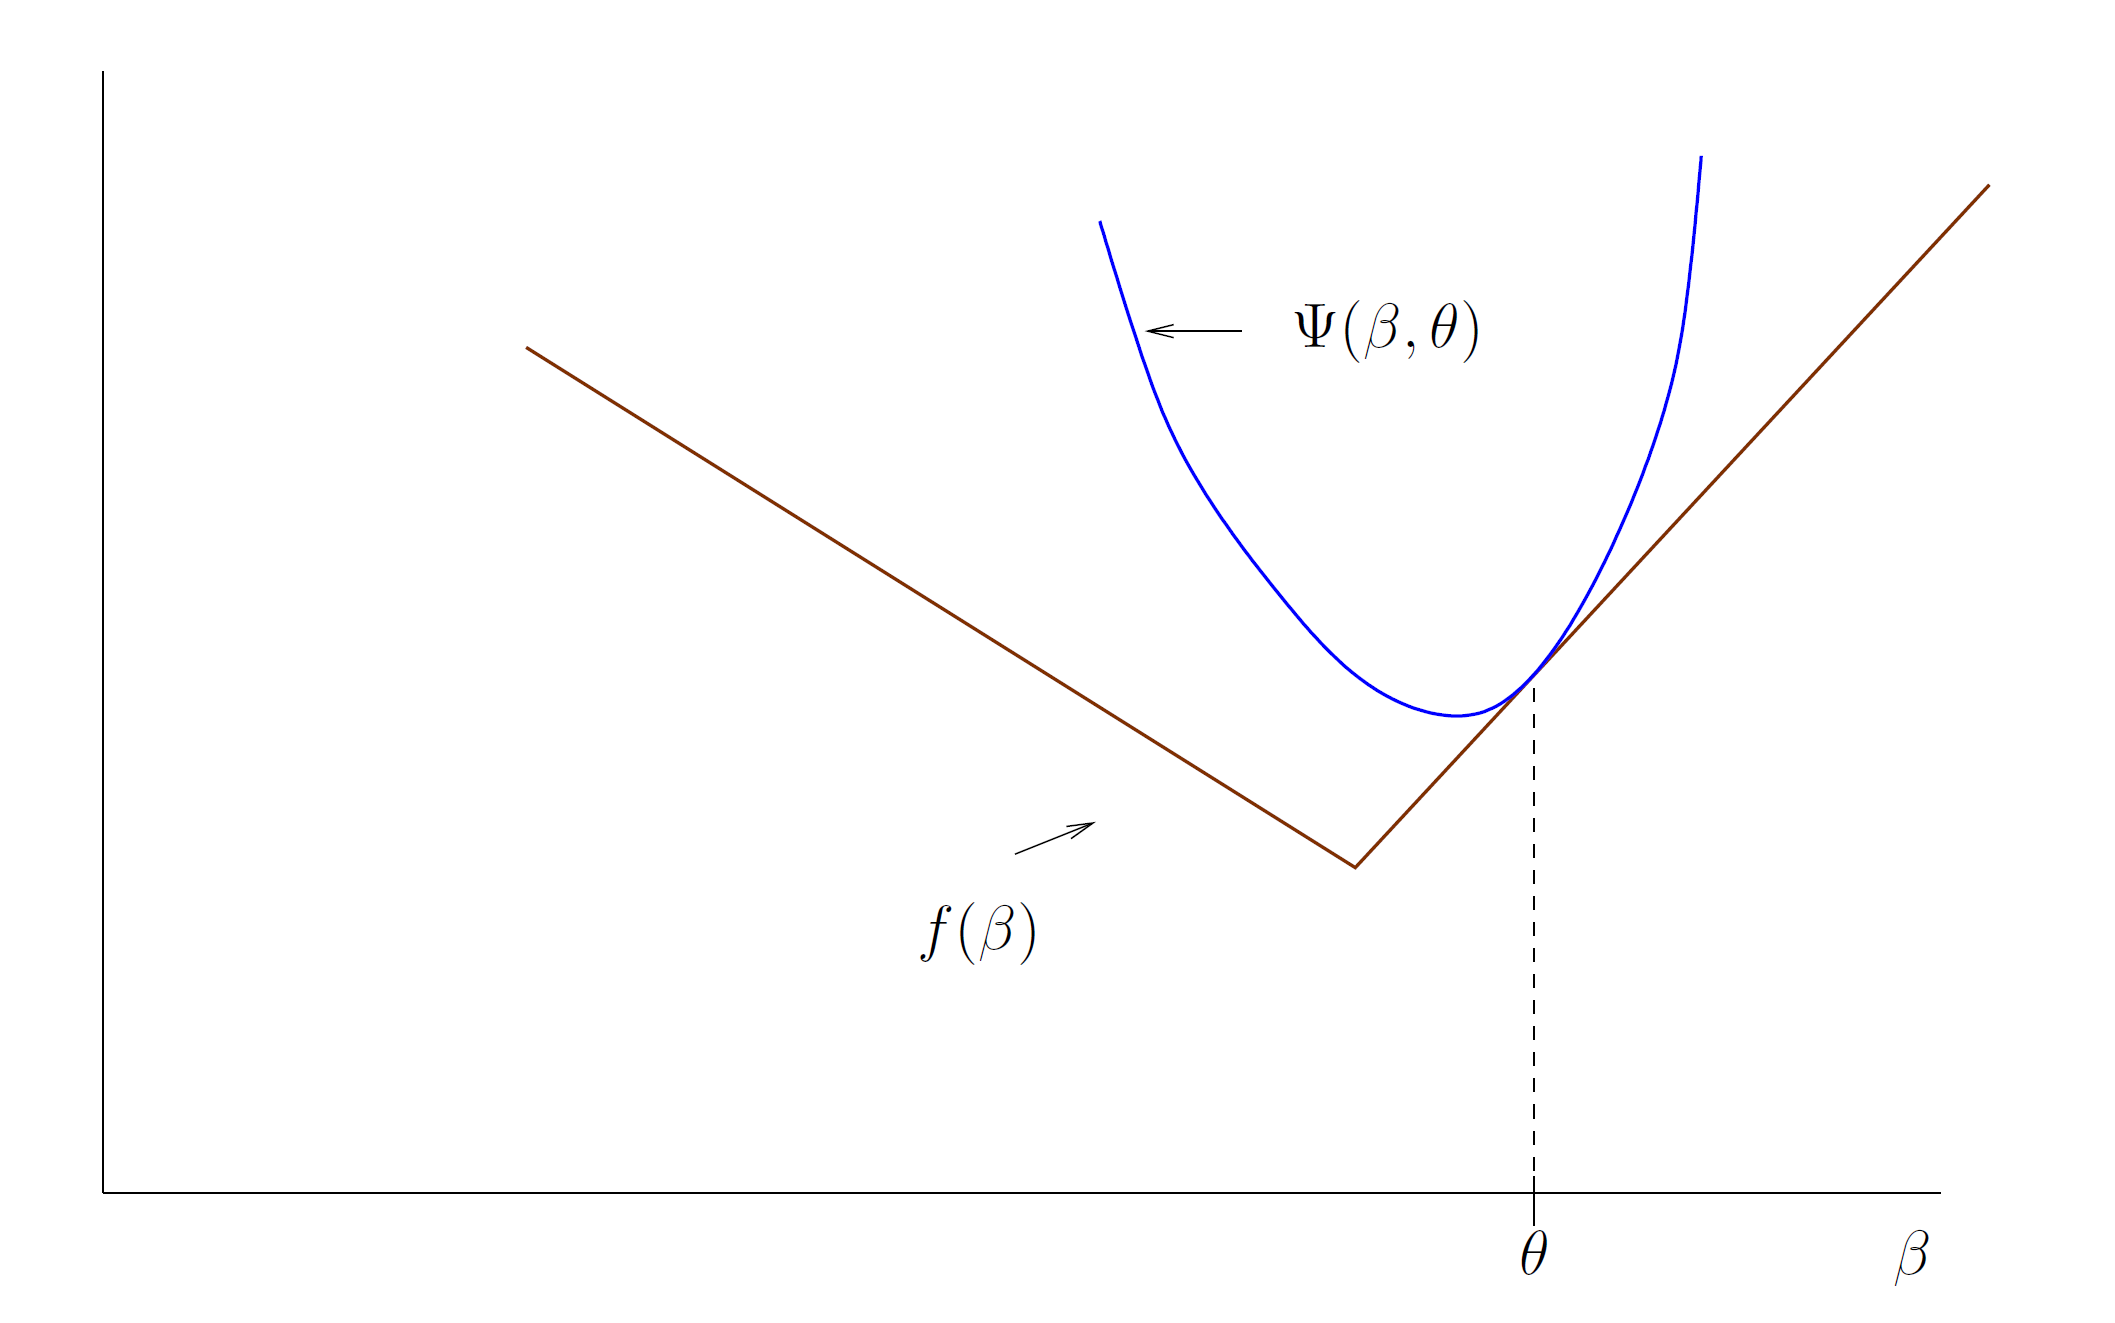
\includegraphics[width=\textwidth]{img/minmaxalgo.png}
%\caption{Figure 5.10 from \cite{Has15}}
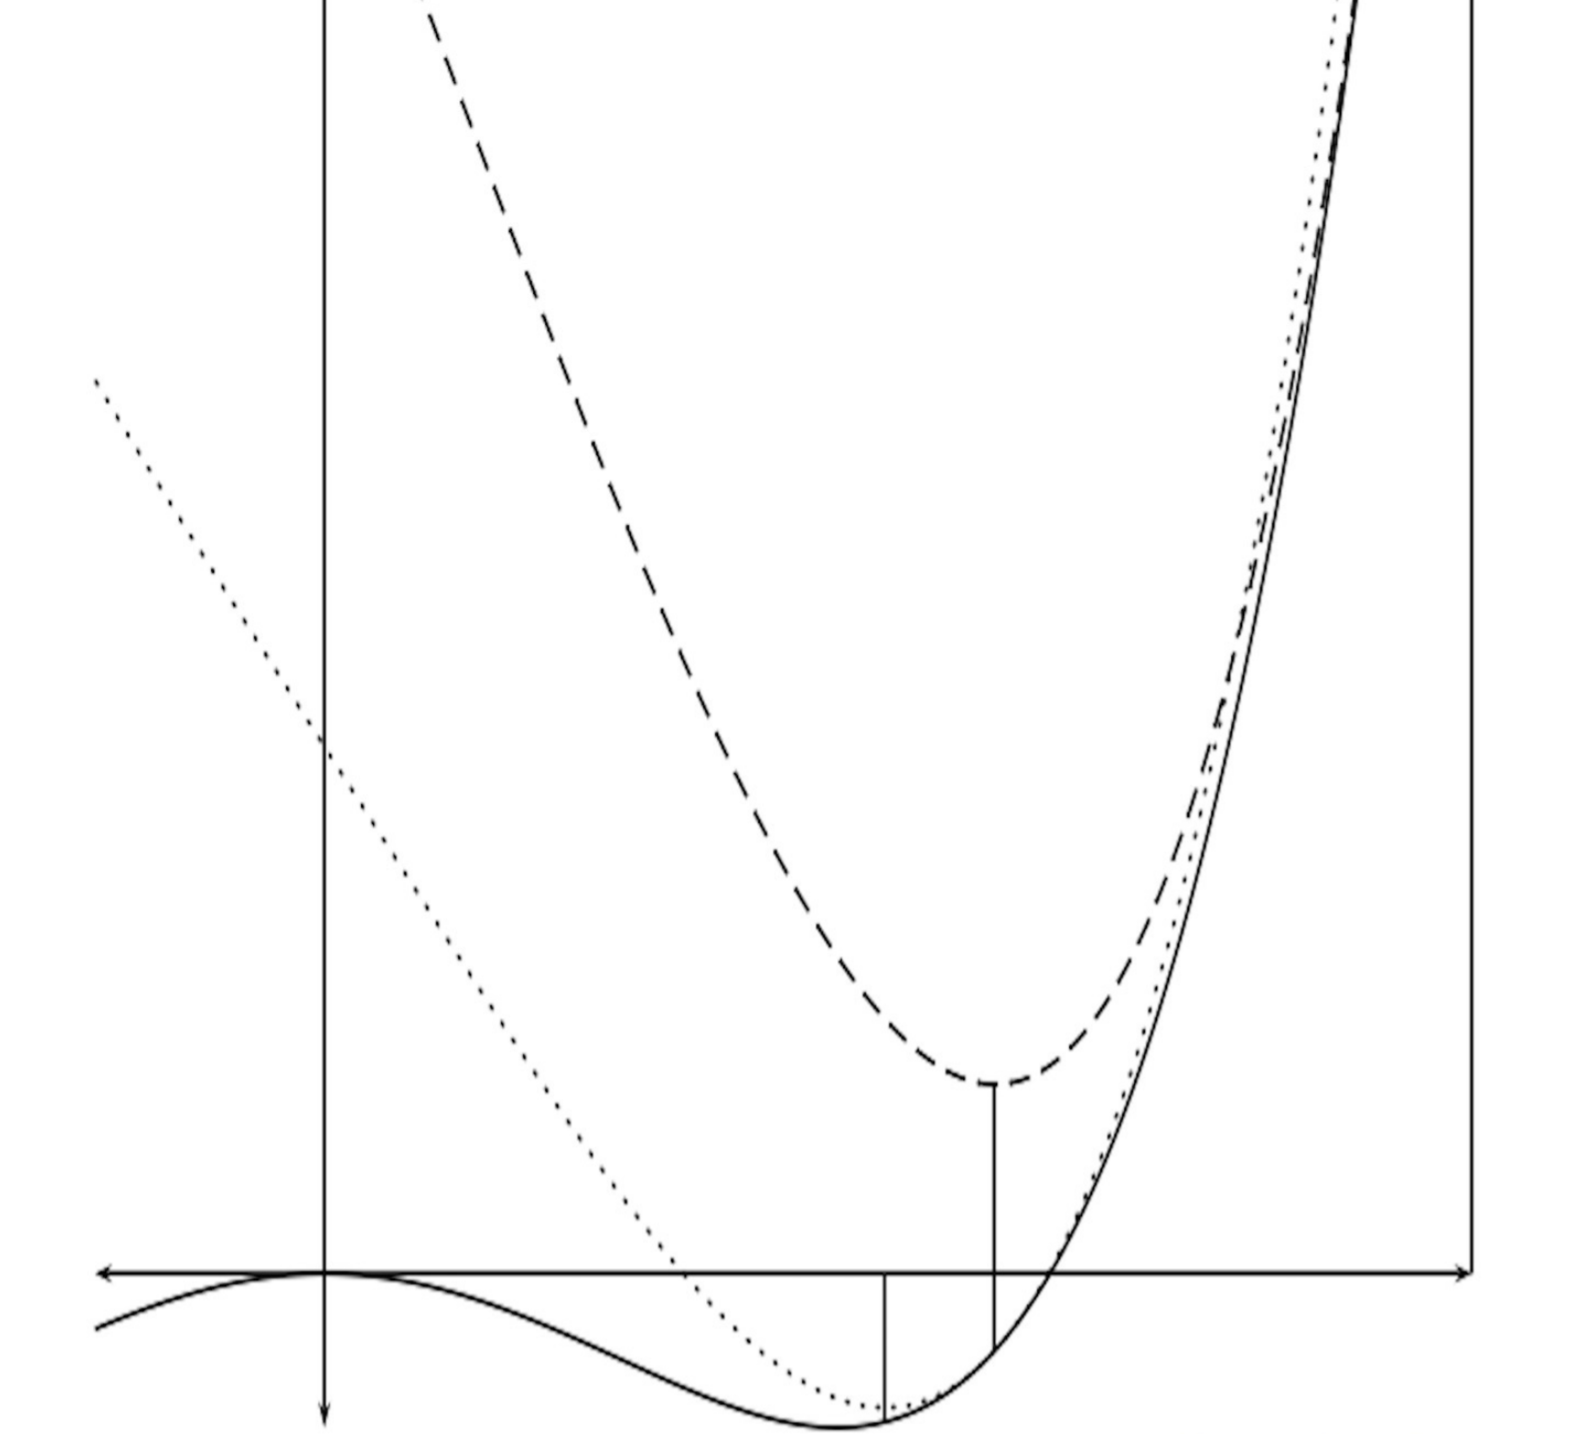
\includegraphics[height=150pt]{img/minmaxalgo2.png}
\caption{Figure from \cite{DL15}}
\end{figure}

\end{frame}

\begin{frame}
\frametitle{MMA analytically I}
Def. 
$\Psi:\R^p\times\R^p\to\R$ {\color{blue}majorizes} $f$ at $\beta\in\R^p$ if \[\forall\theta\in\R^p\quad \Psi(\beta,\theta)\ge f(\beta)\]
with equality for $\theta=\beta$.
\vspace{10pt}

Minor-Maxxalgorithm
\begin{itemize}
\item[-] initialize $\beta^0$
\item[-] update with $\beta^{t+1}=\argmin\limits_{\beta\in\R^p}\Psi(\beta,\beta^t)$
\end{itemize}
\end{frame}

\begin{frame}
\frametitle{MMA analytically II}
This scheme generates a sequence of $\beta$'s for which the cost $f(\beta^t)$ is nonincreasing, because
\[f(\beta^t)\stackrel{(i)}{=}\Psi(\beta^t,\beta^t)\stackrel{(ii)}{\ge}\Psi(\beta^{t+1},\beta^t)\stackrel{(iii)}{\ge} f(\beta^{t+1})\]

where 
\begin{itemize}
\setlength{\itemindent}{20pt}
\item[(i) \& (iii)] Definiton of majorize
\item[(ii)] $\beta^{t+1}$ is a minimizer of $\beta\mapsto\Psi(\beta,\beta^t)$
\end{itemize}
\end{frame}

\note{
for inequalities: show previous slide
}


%------------------------------------------------
\section{Alternating Minimizations}
%------------------------------------------------


\begin{frame}
\frametitle{Biconvexity}
Let's consider an example \dots

\vspace{5pt}
%\url{http://www.wolframalpha.com/input/?i=3D+plot+(1-xy)\%5E2,+x+in+\%5B-2,2\%5D,+y+in+\%5B-2,2\%5D}
{\color{blue}\href{http://www.wolframalpha.com/input/?i=3D+plot+(1-xy)\%5E2,+x+in+\%5B-2,2\%5D,+y+in+\%5B-2,2\%5D}{$f(\alpha,\beta)=(1-\alpha\beta)^2$}}

\note{
Mathematica: \texttt{3D plot (1-xy)\^{}2, x in [-2,2], y in [-2,2]}

The formula is a link.
}

\vspace{30pt}
\only<2>{Def. A function $f(\alpha,\beta):\R^m\times\R^n\to\R$ is {\color{gray}biconvex}, if for each $\alpha\in\R^m$ the function $\alpha\mapsto f(\alpha,\beta)$ is convex  and for each $\beta\in\R^n$ the function $\beta\mapsto f(\alpha,\beta)$ is convex.
\vspace{5pt}
Analoguosly, a set $\mathcal{C}\subseteq\mathcal{A}\times\mathcal{B}$, for $\mathcal{A, B}$ convex sets, is called \underline{biconvex}, if it is convex}
\end{frame}

\begin{frame}
\frametitle{Alternate Convex Search}

Block coordinate descent applied to $\alpha$ and $\beta$ blocks
\begin{enumerate}
\item Initialize $(\alpha^0,\beta^0)$ at some point in the biconvex set to minimize over
\item For $t=0,1,2,\dots$
	\begin{enumerate}[(i)]
	\item Fix $\beta=\beta^t$ and update $\alpha^{t+1}\in\argmin\limits_{\alpha\in\mathcal{C}_{\beta^t}}f(\alpha,\beta^t)$
	\item Fix $\alpha=\alpha^{t+1}$ and update $\beta^{t+1}\in\argmin\limits_{\alpha\in\mathcal{C}_{\alpha^{t+1}}}f(\alpha^{t+1},\beta)$
	\end{enumerate}
\end{enumerate}
\vspace{10pt}

For a function bounded from below, the algorithm converges to a partial optimum (i.e. as biconvexity, only optimal in one coordinate if the other coordinate is fixed).
\end{frame}

%------------------------------------------------
\section{Screening Rules}
%------------------------------------------------

\begin{frame}
\frametitle{Screening Rules}


\end{frame}


\begin{frame}
\frametitle{Dual Polytope Projection (DPP)}
Suppose we want to calculate a lasso solution at $\lambda<\lambda_{\max}$. The DPP rule discards the $j^{th}$ variable if 
\[\norm{\mathbf{x}_j^T\mathbf{y}}<\lambda_{\max}-\Norm{\mathbf{x}_j}_2\Norm{\mathbf{y}}_2\frac{\lambda_{\max}-\lambda}{\lambda}\]

\vspace{5pt}
{\hspace{5pt}\Large Sequential DPP rule}
\vspace{15pt}

Suppose we have the lasso solution $\hat\beta(\lambda')$ at $\lambda'$ and want to screen variables for solutions at $\lambda<\lambda'$. We discard the $j^{th}$ variable if 
\[\norm{\mathbf{x}_j^T(\mathbf{y}-\mathbf{X}\hat{\beta}(\lambda'))}<\lambda'-\Norm{\mathbf{x}_j}_2\Norm{\mathbf{y}}_2\frac{\lambda_{\max}-\lambda}{\lambda}\]
\end{frame}

\begin{frame}
\frametitle{Global Strong Rule}
Suppose we want to calculate a lasso solution at $\lambda<\lambda_{\max}$. The global strong rule discards the $j^{th}$ variable if 
\[\norm{\mathbf{x}_j^T\mathbf{y}}<\lambda-(\lambda_{\max}-\lambda)=2\lambda-\lambda_{\max}\]

\vspace{5pt}
{\hspace{5pt}\Large Sequential Strong Rule}
\vspace{15pt}

Suppose we have the lasso solution $\hat\beta(\lambda')$ at $\lambda'$ and want to screen variables for solutions at $\lambda<\lambda'$. We discard the $j^{th}$ variable if 
\[\norm{\mathbf{x}_j^T(\mathbf{y}-\mathbf{X}\hat{\beta}(\lambda'))}<2\lambda-\lambda'\]
\end{frame}

\begin{frame}
\frametitle{References}
\footnotesize{
\begin{thebibliography}{99} % Beamer does not support BibTeX so references must be inserted manually as below
\bibitem[Hastie et al., 2015]{Has15} Trevor Hastie, Robert Tibshirani, and Martin Wainwright (2015)
\newblock Statistical learning with sparsity: the Lasso and
generalizations
\newblock \emph{CRC Press;} Boca Raton, FL%12(3), 45 -- 678.
\bibitem[de Leeuw, 2015]{DL15} Jan De Leeuw (2015)
\newblock Block Relaxation Methods in Statistics
\newblock \url{doi.org/10.13140/RG.2.1.3101.9607} (last accessed: 02.10.18)
%\bibitem[de Leeuw, 2015]{DL15} Jan De Leeuw (2015)
%\newblock Block Relaxation Methods in Statistics
%\newblock \url{doi.org/10.13140/RG.2.1.3101.9607} (last accessed: 02.10.18)
\bibitem[Gordon and Tibshirani, 2012]{GT12} Geoff Gordon and Ryan Tibshirani (2012)
\newblock Uses of Duality
\newblock \url{https://www.cs.cmu.edu/~ggordon/10725-F12/slides/18-dual-uses.pdf} (last accessed: 14.10.18) 
\end{thebibliography}
}
\end{frame}
%Source: Trevor Hastie, Robert Tibshirani, and Martin Wainwright. Statistical learning with sparsity: the Lasso and generalizations. CRC Press, 2015.
%@unknown{unknown,
%author = {De Leeuw, Jan},
%year = {2015},
%month = {12},
%pages = {},
%title = {Block Relaxation Methods in Statistics - Part II}
%}

%------------------------------------------------
\begin{frame}
\Huge{\centerline{Comments \dots}}
\Huge{\centerline{Questions \dots}}
\Huge{\centerline{Suggestions \dots}}
\end{frame}


\begin{frame}
\Huge{\centerline{That's it.}}
\Huge{\centerline{Thanks for listening.}}
\vspace{20pt}
\large{\centerline{Fill out your feedback sheets!}}
%\Huge{\centerline{The End}}
\end{frame}

%----------------------------------------------------------------------------------------




% ------------------------------------------------------------
%   Everything that is commented below are sample slides from the original template. 
%-------------------------------------------------------------

%
%
%
%\begin{frame}
%\frametitle{Paragraphs of Text}
%Sed iaculis dapibus gravida. Morbi sed tortor erat, nec interdum arcu. Sed id lorem lectus. Quisque viverra augue id sem ornare non aliquam nibh tristique. Aenean in ligula nisl. Nulla sed tellus ipsum. Donec vestibulum ligula non lorem vulputate fermentum accumsan neque mollis.\\~\\
%
%Sed diam enim, sagittis nec condimentum sit amet, ullamcorper sit amet libero. Aliquam vel dui orci, a porta odio. Nullam id suscipit ipsum. Aenean lobortis commodo sem, ut commodo leo gravida vitae. Pellentesque vehicula ante iaculis arcu pretium rutrum eget sit amet purus. Integer ornare nulla quis neque ultrices lobortis. Vestibulum ultrices tincidunt libero, quis commodo erat ullamcorper id.
%\end{frame}
%
%%------------------------------------------------
%
%\begin{frame}
%\frametitle{Bullet Points}
%\begin{itemize}
%\item Lorem ipsum dolor sit amet, consectetur adipiscing elit
%\item Aliquam blandit faucibus nisi, sit amet dapibus enim tempus eu
%\item Nulla commodo, erat quis gravida posuere, elit lacus lobortis est, quis porttitor odio mauris at libero
%\item Nam cursus est eget velit posuere pellentesque
%\item Vestibulum faucibus velit a augue condimentum quis convallis nulla gravida
%\end{itemize}
%\end{frame}
%
%%------------------------------------------------
%
%\begin{frame}
%\frametitle{Blocks of Highlighted Text}
%\begin{block}{Block 1}
%Lorem ipsum dolor sit amet, consectetur adipiscing elit. Integer lectus nisl, ultricies in feugiat rutrum, porttitor sit amet augue. Aliquam ut tortor mauris. Sed volutpat ante purus, quis accumsan dolor.
%\end{block}
%
%\begin{block}{Block 2}
%Pellentesque sed tellus purus. Class aptent taciti sociosqu ad litora torquent per conubia nostra, per inceptos himenaeos. Vestibulum quis magna at risus dictum tempor eu vitae velit.
%\end{block}
%
%\begin{block}{Block 3}
%Suspendisse tincidunt sagittis gravida. Curabitur condimentum, enim sed venenatis rutrum, ipsum neque consectetur orci, sed blandit justo nisi ac lacus.
%\end{block}
%\end{frame}
%
%%------------------------------------------------
%
%\begin{frame}
%\frametitle{Multiple Columns}
%\begin{columns}[c] % The "c" option specifies centered vertical alignment while the "t" option is used for top vertical alignment
%
%\column{.45\textwidth} % Left column and width
%\textbf{Heading}
%\begin{enumerate}
%\item Statement
%\item Explanation
%\item Example
%\end{enumerate}
%
%\column{.5\textwidth} % Right column and width
%Lorem ipsum dolor sit amet, consectetur adipiscing elit. Integer lectus nisl, ultricies in feugiat rutrum, porttitor sit amet augue. Aliquam ut tortor mauris. Sed volutpat ante purus, quis accumsan dolor.
%
%\end{columns}
%\end{frame}
%
%
%\begin{frame}
%\frametitle{Table}
%\begin{table}
%\begin{tabular}{l l l}
%\toprule
%\textbf{Treatments} & \textbf{Response 1} & \textbf{Response 2}\\
%\midrule
%Treatment 1 & 0.0003262 & 0.562 \\
%Treatment 2 & 0.0015681 & 0.910 \\
%Treatment 3 & 0.0009271 & 0.296 \\
%\bottomrule
%\end{tabular}
%\caption{Table caption}
%\end{table}
%\end{frame}
%
%%------------------------------------------------
%
%\begin{frame}
%\frametitle{Theorem}
%\begin{theorem}[Mass--energy equivalence]
%$E = mc^2$
%\end{theorem}
%\end{frame}
%
%%------------------------------------------------
%
%\begin{frame}[fragile] % Need to use the fragile option when verbatim is used in the slide
%\frametitle{Verbatim}
%\begin{example}[Theorem Slide Code]
%\begin{verbatim}
%\begin{frame}
%\frametitle{Theorem}
%\begin{theorem}[Mass--energy equivalence]
%$E = mc^2$
%\end{theorem}
%\end{frame}\end{verbatim}
%\end{example}
%\end{frame}
%
%%------------------------------------------------
%
%\begin{frame}
%\frametitle{Figure}
%Uncomment the code on this slide to include your own image from the same directory as the template .TeX file.
%%\begin{figure}
%%\includegraphics[width=0.8\linewidth]{test}
%%\end{figure}
%\end{frame}
%
%%------------------------------------------------
%
%\begin{frame}[fragile] % Need to use the fragile option when verbatim is used in the slide
%\frametitle{Citation}
%An example of the \verb|\cite| command to cite within the presentation:\\~
%
%This statement requires citation \cite{Has15}.
%\end{frame}

%------------------------------------------------


\end{document} 